\documentclass[11pt,a4paper]{article}
\usepackage[utf8]{inputenc}    % Codificación UTF-8 (obligatorio)
\usepackage[T1]{fontenc}       % Soporte para caracteres europeos
\usepackage[spanish]{babel}    % Idioma español (para guiones y nombres)
\usepackage{float}
\usepackage{graphicx}
\usepackage{parskip} 
\usepackage[a4paper, margin=2cm]{geometry}
\usepackage{setspace}
\usepackage{xcolor} 
\usepackage[most]{tcolorbox}
\usepackage{listings}
\usepackage{enumitem} % <-- Para mejor control de listas
\usepackage{inconsolata} % Fuente moderna monoespaciada
\usepackage{fontawesome5} % Para iconos
\usepackage{calc}
\usepackage{hyperref}
%%% Tabla: 
\usepackage{makecell}       % Para formatear mejor las celdas
\usepackage{multirow}       % Para celdas de múltiples filas
\usepackage{booktabs}       % Mejores líneas horizontales para tablas
\usepackage{colortbl}       % Para colorear celdas
% Definición de colores corporativos (ajústalos según tu preferencia)
\definecolor{headercolor}{RGB}{42, 55, 139}       % Azul oscuro para encabezados
\definecolor{rowcolor1}{RGB}{235, 241, 250}       % Azul muy claro para filas alternas
\definecolor{rowcolor2}{RGB}{255, 255, 255}       % Blanco para filas alternas

% Definición del estilo de cabecera
\newcommand{\headerStyle}[1]{\textcolor{white}{\textbf{#1}}}
% Preambulo para mayor control de las listas de requerimientos funcionales: 
\newcommand{\reqnum}[1]{\textbf{\underline{RF-#1}}}
% Estilo para elementos futuros
\newcommand{\future}[1]{\textit{#1}}


\setstretch{1.2}
% Definir colores modernos
\definecolor{background}{RGB}{250, 250, 252}
\definecolor{comment}{RGB}{92, 122, 158}
\definecolor{keyword}{RGB}{130, 80, 223}
\definecolor{string}{RGB}{64, 160, 112}
\definecolor{number}{RGB}{209, 105, 105}
\definecolor{identifier}{RGB}{36, 41, 46}
\definecolor{frame}{RGB}{232, 234, 237}
\definecolor{caption}{RGB}{42, 44, 57}

% Estilo para JSON
\lstdefinelanguage{json}{
    basicstyle=\fontfamily{zi4}\selectfont\footnotesize,
    commentstyle=\color{comment}\itshape,
    keywordstyle=\color{keyword}\bfseries,
    numberstyle=\tiny\color{number},
    stringstyle=\color{string},
    breakatwhitespace=false,
    breaklines=true,
    keepspaces=true,
    numbers=left,
    numbersep=10pt,
    showspaces=false,
    showstringspaces=false,
    showtabs=false,
    tabsize=2,
    morestring=[b]",
    morekeywords={true,false,null}
}

% Estilo para HTTP
\lstdefinelanguage{HTTP}{
    morekeywords={GET,POST,PUT,DELETE,HEAD,OPTIONS,PATCH},
    sensitive=false,
    morecomment=[l]{//},
    morecomment=[s]{/*}{*/},
    morestring=[b]",
    basicstyle=\fontfamily{zi4}\selectfont\footnotesize\color{identifier},
    keywordstyle=\color{keyword}\bfseries,
}

% Estilo para JavaScript
\lstdefinelanguage{JavaScript}{
    keywords={typeof, new, true, false, catch, function, return, null, catch, switch, var, if, in, while, do, else, case, break},
    keywordstyle=\color{keyword}\bfseries,
    ndkeywords={class, export, boolean, throw, implements, import, this},
    ndkeywordstyle=\color{number}\bfseries,
    identifierstyle=\color{identifier},
    sensitive=false,
    comment=[l]{//},
    morecomment=[s]{/*}{*/},
    morestring=[b]',
    morestring=[b]",
    basicstyle=\fontfamily{zi4}\selectfont\footnotesize\color{identifier},
}

% Definir entorno personalizado para los bloques de código
\newtcolorbox{codebox}[2][]{
    colback=background,
    colframe=frame,
    boxrule=1pt,
    title=#2,
    before skip=10pt,
    after skip=10pt,
    #1
}

% Configuración global para listings
\lstset{
    basicstyle=\fontfamily{zi4}\selectfont\footnotesize\color{identifier},
    commentstyle=\color{comment},
    breaklines=true,
    backgroundcolor=\color{background},
    frame=none,
    framesep=5pt,
    xleftmargin=15pt,
    numbers=left,
    numberstyle=\tiny\color{comment},
    stepnumber=1,
    numbersep=10pt,
    captionpos=t,
}


\title{Documento de arquitectura y desarrollo del sistema SID}
\author{Henry Ricaurte Mora}
\date{Abril de 2025}

\begin{document}

\maketitle

\tableofcontents

\newpage

\section{Introducción}

En esta sección se brinda una visión introductoria de los conceptos relacionados con la descripción del sistema del SID.
Es importante establecer una estructura clara de los componentes que lo conforman.

\begin{figure}[htbp]
	\centering
	\includegraphics[width=0.8\textwidth]{src/SID_org.pdf}
	\caption{Diagrama de organización del SID}
\end{figure}

El SID está conformado por tres ramas principales:

\begin{itemize}
	\item \textbf{Desarrollos:} Social, Robótico y Web.
	\item \textbf{Comités:} Financiera, Logística, Apoyo, Marketing y Desarrollo.
	\item \textbf{Participantes:} \textit{Partners} y \textit{Members}.
\end{itemize}

\subsection{Comités}

Los comités son responsables del funcionamiento del SID. Cada uno tiene un presidente y un vicepresidente,
quienes lideran al equipo para desarrollar estrategias como:

\begin{itemize}
	\item Generar ingresos para financiar proyectos.
	\item Organizar la logística de las actividades.
	\item Establecer dinámicas de formación para los integrantes.
	\item Crear contenido audiovisual para promoción.
	\item Supervisar y respaldar a los grupos de desarrollo.
\end{itemize}

\subsection{Desarrollos}

Cada desarrollo (Social, Robótico y Web) cuenta con un líder, sublíderes y un equipo.
El líder coordina el proyecto general, los sublíderes gestionan apartados específicos y los integrantes trabajan bajo su guía.

Por ejemplo, este documento forma parte de un proyecto en el desarrollo Web.

\paragraph{}
Los \textit{Partners} incluyen a presidentes, vicepresidentes, líderes y sublíderes. Los \textit{Members} son
integrantes que participan activamente en cada uno de los apartados de desarrollo.

\section{Descripción General del Sistema}
Se desarrollará una plataforma integral para la gestión y difusión de información del grupo SID. Esta incluirá herramientas para la presentación institucional, la oferta de cursos de formación y la divulgación de conocimiento especializado.

\subsection{Componentes Principales}
\begin{itemize}
	\item \textbf{Portal Web Principal: } Será el sitio informativo del grupo,
	      donde se mostrará quiénes somos y cuáles son nuestras áreas de trabajo. Este portal incluirá secciones dedicadas a los distintos
	      desarrollos del grupo, cada una con su propia página que detallará a sus integrantes, proyectos y líderes. Asimismo, se presentarán los
	      comités con una estructura similar.
	      También se incluirá información general sobre el SID, sus actividades, proyectos, equipos, colaboraciones, cursos, noticias e integrantes,
	      además de un formulario de inscripción para nuevos miembros o interesados.

	\item \textbf{Panel Administrativo: } Permitirá la gestión del contenido visible en el portal principal, así como la administración de los datos de los usuarios provenientes de los formularios de inscripción.

	\item \textbf{Sistema de Gestión Académica: } Este componente permitirá la inscripción y administración de los cursos ofrecidos. Incluirá funcionalidades específicas para tres tipos de usuarios: administrador, profesor y estudiante/usuario. También facilitará la asignación y gestión de profesores por curso.

	\item \textbf{SID Academy: } Proyecto futuro que se plantea como una plataforma educativa de cursos breves, similar a QtAcademy, con el objetivo de fortalecer el aprendizaje especializado dentro de la comunidad.
\end{itemize}

\section{Requerimientos del Sistema}
\subsection{Requerimientos Funcionales: }
\subsubsection{Portal Web Principal}
\begin{enumerate}[leftmargin=*,labelwidth=2.5cm,align=left]
	\item[\reqnum{001}] El sistema debe mostrar información institucional del grupo SID.
	\item[\reqnum{002}] El sistema debe presentar secciones para cada desarrollo del grupo (Web, Robótica, Social) con sus integrantes, proyectos y líderes.
	\item[\reqnum{003}] El sistema debe mostrar información sobre los comités existentes.
	\item[\reqnum{004}] El sistema debe listar actividades realizadas por el grupo.
	\item[\reqnum{005}] El sistema debe mostrar proyectos desarrollados por el grupo.
	\item[\reqnum{006}] El sistema debe exponer los cursos ofrecidos por el grupo.
	\item[\reqnum{007}] El sistema debe presentar los equipos de trabajo.
	\item[\reqnum{008}] El sistema debe publicar noticias relacionadas con el grupo.
	\item[\reqnum{009}] El sistema debe mostrar información sobre fundaciones y colaboraciones.
	\item[\reqnum{010}] El sistema debe incluir un formulario de inscripción para nuevos miembros.
\end{enumerate}

\subsubsection{Panel Administrativo (Dashboard)}
\begin{enumerate}[leftmargin=*,labelwidth=2.5cm,align=left,start=11]
	\item[\reqnum{011}] El sistema debe permitir a los administradores gestionar el contenido del portal web.
	\item[\reqnum{012}] El sistema debe proporcionar funcionalidades para administrar los datos de usuarios.
	\item[\reqnum{013}] El sistema debe permitir la gestión de actividades (crear, modificar, eliminar).
	\item[\reqnum{014}] El sistema debe permitir la gestión de proyectos (crear, modificar, eliminar).
	\item[\reqnum{015}] El sistema debe permitir la gestión de cursos (crear, modificar, eliminar).
	\item[\reqnum{016}] El sistema debe permitir la gestión de equipos (crear, modificar, eliminar).
	\item[\reqnum{017}] El sistema debe permitir la gestión de noticias (crear, modificar, eliminar).
	\item[\reqnum{018}] El sistema debe permitir la gestión de fundaciones (crear, modificar, eliminar).
	\item[\reqnum{019}] El sistema debe implementar control de acceso basado en roles.
	\item[\reqnum{020}] El sistema debe permitir la administración de permisos por rol.
\end{enumerate}

\subsubsection{API de Servicios}
\begin{enumerate}[leftmargin=*,labelwidth=2.5cm,align=left,start=21]
	\item[\reqnum{021}] El sistema debe proporcionar endpoints RESTful para listar contenido (actividades, proyectos, etc.).
	\item[\reqnum{022}] El sistema debe implementar paginación en todos los endpoints que devuelven listas.
	\item[\reqnum{023}] El sistema debe manejar formatos estándar para solicitudes y respuestas (JSON).
	\item[\reqnum{024}] El sistema debe implementar autenticación mediante tokens JWT.
	\item[\reqnum{025}] El sistema debe proporcionar endpoints para la gestión de contenidos protegidos por autenticación.
\end{enumerate}

\subsection{Requerimientos No Funcionales}

\subsubsection{Seguridad}
\begin{enumerate}[leftmargin=*,labelwidth=2.5cm,align=left]
	\item[\reqnum{026}] El sistema debe implementar autenticación OAuth 2.0 con proveedores de identidad externos (Microsoft Entra ID/Azure AD / Google).
	\item[\reqnum{027}] El sistema debe validar y procesar tokens JWT emitidos por el proveedor de identidad.
	\item[\reqnum{028}] El sistema debe implementar control de acceso basado en roles mediante la base de datos
	\item[\reqnum{029}] El sistema debe proteger los endpoints administrativos con autorización basada en roles
	\item[\reqnum{030}] El sistema debe usar HTTPS para todas las comunicaciones (TLS 1.2+). | Toca entender que es a profundidad
	\item[\reqnum{031}] El sistema debe implementar protección contra ataques comunes (CSRF, XSS, SQL Injection).
\end{enumerate}

\subsubsection{Rendimiento}
\begin{enumerate}[leftmargin=*,labelwidth=2.5cm,align=left,start=32]
	\item[\reqnum{032}] El sistema debe responder a las solicitudes API en menos de 1 segundo bajo carga normal.
	\item[\reqnum{033}] El sistema debe soportar al menos 100 usuarios concurrentes.
	\item[\reqnum{034}] Las consultas a la base de datos deben optimizarse para minimizar el tiempo de respuesta.
\end{enumerate}

\subsubsection{Escalabilidad}
\begin{enumerate}[leftmargin=*,labelwidth=2.5cm,align=left,start=35]
	\item[\reqnum{035}] La arquitectura debe permitir escalar componentes individuales según demanda.
	\item[\reqnum{036}] El sistema debe ser compatible con despliegue en contenedores (Docker/Kubernetes).
\end{enumerate}

\subsubsection{Mantenibilidad}
\begin{enumerate}[leftmargin=*,labelwidth=2.5cm,align=left,start=37]
	\item[\reqnum{037}] El código debe seguir los principios SOLID y patrones de diseño apropiados.
	\item[\reqnum{038}] El sistema debe implementar logging estructurado (JSON) para diagnóstico.
	\item[\reqnum{039}] El código debe incluir documentación JavaDoc y OpenAPI para las APIs.
\end{enumerate}

\subsubsection{Compatibilidad}
\begin{enumerate}[leftmargin=*,labelwidth=2.5cm,align=left,start=40]
	\item[\reqnum{040}] Las APIs deben seguir el estándar RESTful nivel 2 de Richardson.
	\item[\reqnum{041}] El sistema debe proporcionar documentación interactiva mediante Swagger UI.
\end{enumerate}

\subsubsection{Interoperabilidad}
\begin{enumerate}[leftmargin=*,labelwidth=2.5cm,align=left,start=44]
	\item[\reqnum{044}] El sistema debe exponer APIs con versionado semántico (v1, v2). | Acordar si mandarlo en header o en la api. (obligatorio tag github)
	\item[\reqnum{045}] Las integraciones deben usar protocolos estándar (OAuth 2.0, OpenID Connect).
\end{enumerate}



\section{Especificación Modulos:}

\begin{figure}[H]
	\centering
	\includegraphics[width=0.5\textwidth]{src/SID_microservices.pdf}
	\caption{Diagrama de microservicios del proyecto}
\end{figure}

\section*{Microservicios propuestos}

\subsection{Servicio de Autenticación y Usuarios}
\begin{itemize}
	\item Gestión completa del ciclo de vida de usuarios
	\item Autenticación y autorización
	\item Gestión de tokens y sesiones
\end{itemize}

\subsection{Servicio de Estructura Organizacional}
\begin{itemize}
	\item Visualización de desarrollos (Web, Robótica, etc.)
	\item Visualización de comités (Financiero, Social, etc.)
	\item Visualización de noticias y actualizaciones
	\item Visualización de información sobre fundaciones y trabajos realizados
	\item Visualización de integrantes y Formulario

	\item Administración y gestión de desarrollos (Web, Robótica, etc.)
	\item Administración y gestión de comités (Financiero, Social, etc.)
	\item Administración y gestión de noticias y actualizaciones
	\item Administración y gestión de información sobre fundaciones y trabajos realizados
	\item Administración y gestión de integrantes
	\item Administracion de integrantes mediante Formulario.
\end{itemize}

\subsection{Servicio de Gestión Académica}
\begin{itemize}
	\item Catálogo e inscripción a cursos
	\item Gestión de profesores y alumnos
	\item Seguimiento y evaluación
\end{itemize}

\subsection{Servicio QtAcademy (futuro)}
\begin{itemize}
	\item Gestión de contenidos educativos cortos
	\item Sistema de aprobación y curación
	\item Análisis de métricas de consumo
\end{itemize}


\begin{table}[H]
	\centering
	\renewcommand{\arraystretch}{1.5}
	\begin{tabular}{>{\raggedright\arraybackslash}p{2.8cm} >{\raggedright\arraybackslash}p{5.0cm} >{\raggedright\arraybackslash}p{3.0cm} >{\raggedright\arraybackslash}p{3.0cm}}
		\toprule
		\rowcolor{headercolor}
		\headerStyle{M{\'o}dulo}                   & \headerStyle{Función principal} & \headerStyle{Métodos API} & \headerStyle{Seguridad} \\
		\midrule
		\rowcolor{rowcolor1}
		\textbf{AuthService}                       &
		Autenticación y autorización\newline
		Gestión de usuarios y roles\newline
		Administración de tokens y sesiones        &
		\begin{itemize}[nosep,leftmargin=*]
			\item POST
			\item GET
			\item PUT
		\end{itemize}        &
		JWT\newline
		(Solo login es público)                                                                                                            \\
		\midrule
		\rowcolor{rowcolor2}
		\textbf{PortalService y Dashboard control} &
		Visualización pública del SID\newline
		(desarrollos, comités, noticias)\newline
		Administración de desarrollos\newline
		Gestión de comités y fundaciones           &
		\begin{itemize}[nosep,leftmargin=*]
			\item GET
			\item POST
			\item PUT
			\item PATCH
			\item DELETE
		\end{itemize}        &
		Mixto:\newline
		• Público (lectura)\newline
		• JWT + roles (escritura)                                                                                                          \\
		\midrule
		\rowcolor{rowcolor1}
		\textbf{CoursesService}                    &
		Gestión de cursos e inscripciones\newline
		Administración de profesores/alumnos\newline
		Seguimiento y evaluación académica         &
		\begin{itemize}[nosep,leftmargin=*]
			\item GET
			\item POST
			\item PUT
		\end{itemize}        &
		JWT + roles\newline
		(basado en perfiles académicos)                                                                                                    \\
		\midrule
		\rowcolor{rowcolor2}
		\textbf{\future{SIDAcademy}}\newline
		\textit{(futuro)}                          &
		Contenidos educativos cortos\newline
		Curación de material didáctico\newline
		Análisis de métricas de aprendizaje        &
		\begin{itemize}[nosep,leftmargin=*]
			\item GET
			\item POST
			\item PUT
		\end{itemize}        &
		JWT + roles\newline
		(según nivel de acceso)                                                                                                            \\
		\bottomrule
	\end{tabular}
	\caption{Arquitectura de modulos propuesta para el sistema SID}
\end{table}
\section{Arquitectura de Base de Datos: }
Como base de datos se elige una NewSQL como Neon la cual opera con postgresql, elegido por comidad de diseño y ademas brinda lo necesario para el proyecto.
La base de datos generada es:
\begin{figure}[H]
	\centering
	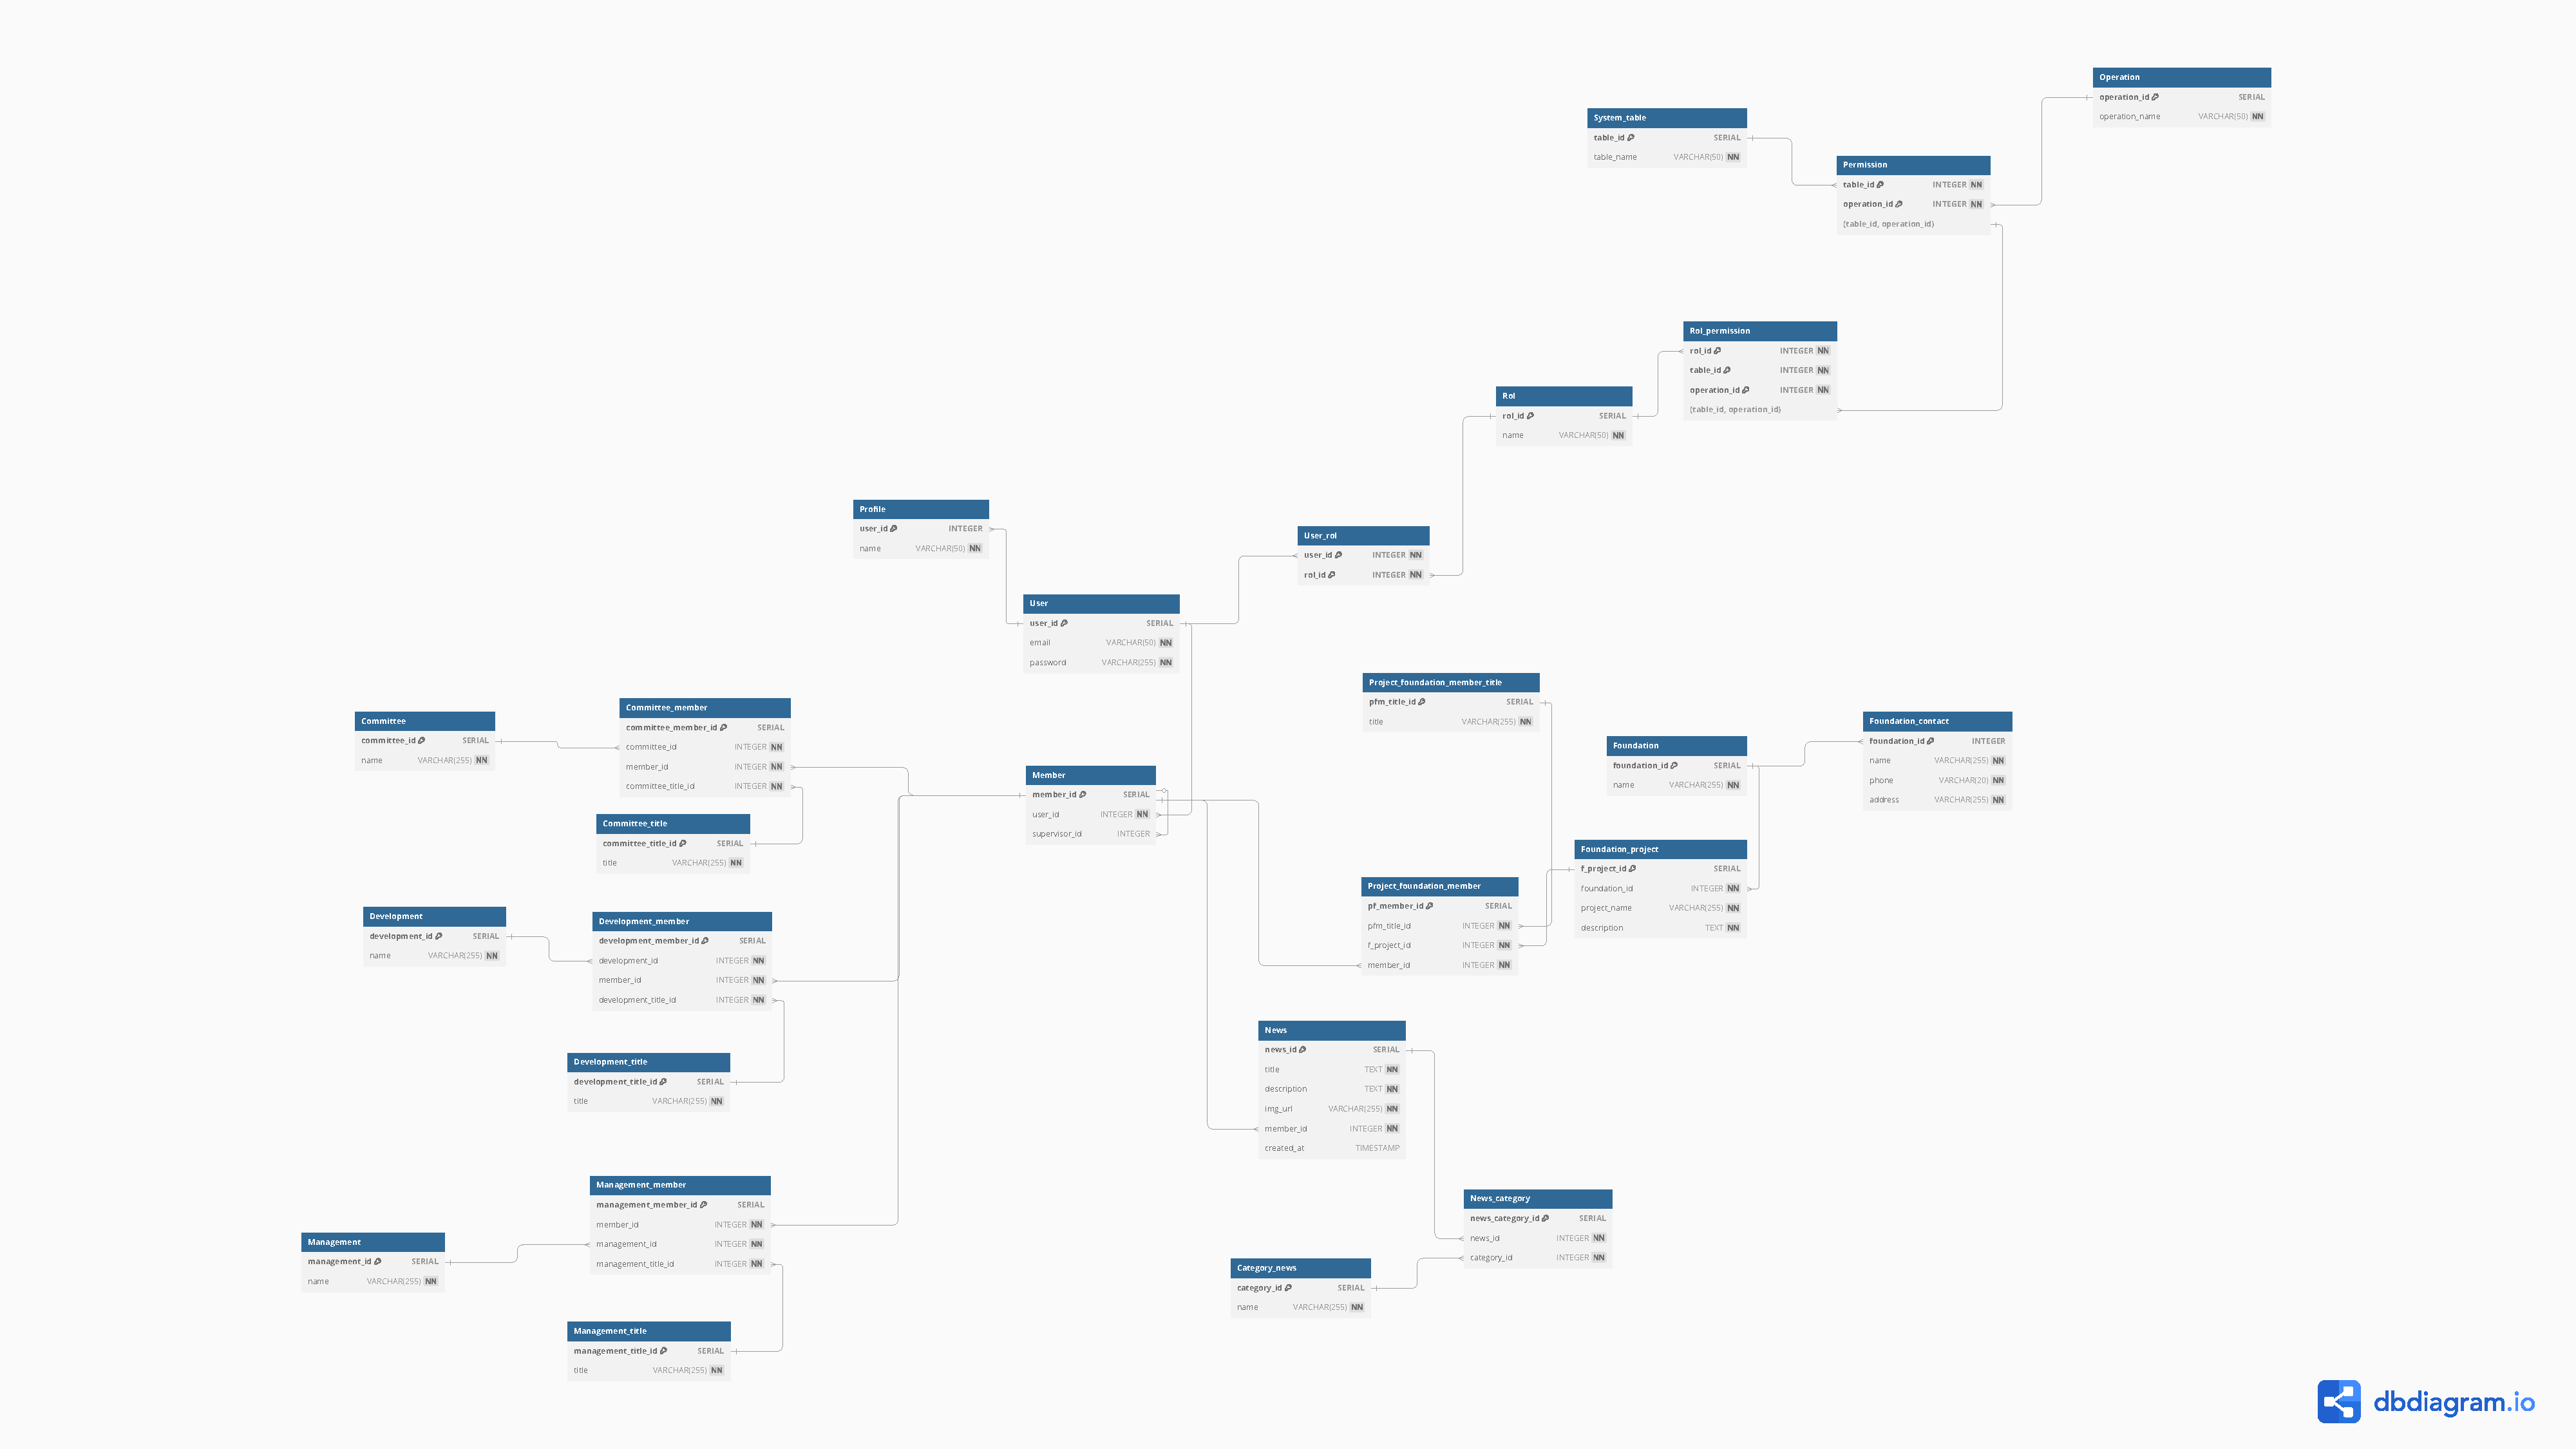
\includegraphics[width=0.5\textwidth]{src/SID_Db.pdf}
	\caption{Diagrama de base de datos relacional}
\end{figure}
\begin{figure}[H]
	\centering
	\includegraphics[width=0.5\textwidth]{src/Modelo-pica.png}
	\caption{Diagrama de base de datos relacional desde google}
\end{figure}
\section{Arquitectura de modulos y microservicios: }
Vamos a abordar todo el tema de los m{\'o}dulos y microservicios ademas de su arquitectura paso por paso.
El único microservicio actual es AuthService, luego estan los m{\'o}dulos monoliticos como el \textbf{Portal Content Service}
\section{Portal Content Service}
Este servicio de portal de contenido que se generará es la dicha ``Página del SID'', desde el lado del backend tenemos que suplir información relevante,
esta información está dividida en:
\begin{itemize}
	\item Actividades (no está en BD)
	\item Proyectos (no está en BD)
	\item Cursos (no está en BD) -- final
	\item Equipos (no está en BD)
	\item Noticias
	\item Aliados | Fundaciones
\end{itemize}

\subsection{Endpoints REST}
Con base en los elementos anteriores, definimos los siguientes endpoints REST con paginación de Spring Boot:

%%%%%%%%%%%%%%%%%%%%%%%%%%%%%   ACTIVIDADES %%%%%%%%%%%%%%%%%%%%

\subsubsection{Actividades}

%%%%%%%%%%%%%%%%%%%%%%%%%%%%%   PROYECTOS %%%%%%%%%%%%%%%%%%%%

\subsubsection{Proyectos}

%%%%%%%%%%%%%%%%%%%%%%%%%%%%%   CURSOS %%%%%%%%%%%%%%%%%%%%

\subsubsection{Cursos}

%%%%%%%%%%%%%%%%%%%%%%%%%%%%%   EQUIPOS  %%%%%%%%%%%%%%%%%%%%

\subsubsection{Equipos}

%%%%%%%%%%%%%%%%%%%%%%%%%%%%%   NOTICIAS %%%%%%%%%%%%%%%%%%%%
\subsubsection{Noticias}

\paragraph{GET Todos (Paginado)}

\begin{center}
	\begin{minipage}{\textwidth}
		\begin{codebox}{GET Noticias (paginado)}
			\begin{lstlisting}[language=HTTP]
GET /api/news?page=0&size=10&sort=publishDate,desc
\end{lstlisting}
		\end{codebox}
	\end{minipage}
\end{center}

\begin{center}
	\begin{minipage}{\textwidth}
		\begin{codebox}{Estructura de respuesta}
			\begin{lstlisting}[language=json]
{
    "content": [
        {
            "id": integer,                   // ID unico de la noticia
            "title": string,                 // Titulo de la noticia
            "content": string(HTML),         // Contenido completo en HTML
            "publishDate": string(ISO-8601), // Fecha de publicacion
            "author": string,                // Nombre del autor
            "imageUrl": string(URL),         // Ruta a la imagen destacada
            "tags": string[]                 // Array de etiquetas
        }
        // ... mas elementos
    ],
    "pageable": {
        "sort": object,       // Informacion de ordenamiento
        "pageSize": integer,  // Tamano de pagina solicitado
        "pageNumber": integer // Numero de pagina actual
        // ... mas metadatos de paginacion
    },
    "totalElements": integer, // Total de resultados
    "totalPages": integer,    // Total de paginas disponibles
    "first": boolean,         // Si es la primera pagina
    "last": boolean,          // Si es la ultima pagina
    "size": integer           // Tamano de la pagina actual
}
\end{lstlisting}
		\end{codebox}
	\end{minipage}
\end{center}

\paragraph{GET Individual}

\begin{center}
	\begin{minipage}{\textwidth}
		\begin{codebox}{GET /api/news/{id} - Obtener noticia específica}
			\begin{lstlisting}[language=HTTP]
GET /api/news/{id}
\end{lstlisting}
		\end{codebox}
	\end{minipage}
\end{center}

\begin{center}
	\begin{minipage}{\textwidth}
		\begin{codebox}{Estructura de respuesta}
			\begin{lstlisting}[language=json]
{
    "id": integer,                   // ID unico de la noticia
    "title": string,                 // Titulo de la noticia
    "content": string(HTML),         // Contenido completo en HTML
    "publishDate": string(ISO-8601), // Fecha de publicacion
    "author": string,                // Nombre del autor
    "imageUrl": string(URL),         // Ruta a la imagen destacada
    "tags": string[]                 // Array de etiquetas
}
\end{lstlisting}
		\end{codebox}
	\end{minipage}
\end{center}

\paragraph{POST Creación}
\begin{center}
	\begin{minipage}{\textwidth}
		\begin{codebox}{POST /api/news - Crear nueva noticia}
			\begin{lstlisting}[language=HTTP]
POST /api/news
Content-Type: application/json
Authorization: Bearer <token>

{
    "title": string,       // Requerido: Titulo de la noticia
    "content": string(URL:.MD) // Requerido: Ruta para contenido posiblemente HTML o .MD , en su defecto el contenido en un string
    "tags": string[]  //  Array de etiquetas 
    "imageURL": String(URL) // Ruta a la Imagen
}
\end{lstlisting}
		\end{codebox}
	\end{minipage}
\end{center}

\begin{center}
	\begin{minipage}{\textwidth}
		\begin{codebox}{Estructura de respuesta}
			\begin{lstlisting}[language=json]
{
    "id": integer,                   // ID generado automaticamente
    "title": string,                 // Titulo proporcionado
    "status": string(enum),          // Estado inicial: DRAFT
    "createdAt": string(ISO-8601)    // Timestamp de creacion
}
\end{lstlisting}
		\end{codebox}
	\end{minipage}
\end{center}

\paragraph{PUT (Reemplazo completo)}
\begin{center}
	\begin{minipage}{\textwidth}
		\begin{codebox}{PUT /api/news/{id} - Actualizar noticia completa}
			\begin{lstlisting}[language=HTTP]
PUT /api/news/{id}
Content-Type: application/json
Authorization: Bearer <token>

{
    "title": string,        // Requerido: Nuevo titulo
    "content": string(HTML) // Requerido: Nuevo contenido
    "imageURL": string(URL) // Ruta de la nueva imagen
    // Todos los campos son requeridos en PUT , 
    // se pueden dejar en blanco si no se quiere actualizar ese apartado
}
\end{lstlisting}
		\end{codebox}
	\end{minipage}
\end{center}

\begin{center}
	\begin{minipage}{\textwidth}
		\begin{codebox}{Estructura de respuesta}
			\begin{lstlisting}[language=json]
{
    "id": integer,                   // ID de la noticia actualizada
    "title": string,                 // Titulo actualizado
    "lastUpdated": string(ISO-8601)  // Timestamp de actualizacion
}
\end{lstlisting}
		\end{codebox}
	\end{minipage}
\end{center}

\paragraph{PATCH (Actualización parcial)}
\begin{center}
	\begin{minipage}{\textwidth}
		\begin{codebox}{PATCH /api/news/{id} - Actualizar campos específicos}
			\begin{lstlisting}[language=HTTP]
PATCH /api/news/{id}
Content-Type: application/json-patch+json
Authorization: Bearer <token>

[
    { "op": string(enum), 
      "path": string, 
      "value": any 
    }, // Operacion JSON Patch

    // Operaciones permitidas: "replace", "add", "remove"
    // Ejemplo: { "op": "replace", "path": "/title", "value": "Nuevo titulo" }
]
\end{lstlisting}
		\end{codebox}
	\end{minipage}
\end{center}

\begin{center}
	\begin{minipage}{\textwidth}
		\begin{codebox}{Estructura de respuesta}
			\begin{lstlisting}[language=json]
{
    "id": integer,     // ID de la noticia modificada
    "changes": string[], // Lista de campos modificados
    "version": integer   // Nueva version del documento
}
\end{lstlisting}
		\end{codebox}
	\end{minipage}
\end{center}

\paragraph{DELETE}
\begin{center}
	\begin{minipage}{\textwidth}
		\begin{codebox}{DELETE /api/news/{id} - Eliminar noticia}
			\begin{lstlisting}[language=HTTP]
DELETE /api/news/{id}
Authorization: Bearer <token>
\end{lstlisting}
		\end{codebox}
	\end{minipage}
\end{center}

\begin{center}
	\begin{minipage}{\textwidth}
		\begin{codebox}{Respuesta}
			\begin{lstlisting}[language=HTTP]
HTTP/1.1 204 No Content
// No se devuelve cuerpo de respuesta
\end{lstlisting}
		\end{codebox}
	\end{minipage}
\end{center}


%%%%%%%%%%%%% ALIADOS Y FUNDACIONES %%%%%%%%%%%%%%%%%%%
\subsubsection{Aliados y Fundaciones}

\paragraph{GET Todos (Paginado)}

\begin{center}
	\begin{minipage}{\textwidth}
		\begin{codebox}{GET Aliados (paginado)}
			\begin{lstlisting}[language=HTTP]
GET /api/allies?page=0&size=10&type=FOUNDATION
\end{lstlisting}
		\end{codebox}
	\end{minipage}
\end{center}

\begin{center}
	\begin{minipage}{\textwidth}
		\begin{codebox}{Estructura de respuesta}
			\begin{lstlisting}[language=json]
{
    "content": [
        {
            "id": integer,                   // ID unico del aliado
            "name": string,                  // Nombre de la organizacion
            "type": string(enum),            // Tipo: FOUNDATION, COMPANY, NGO, etc.
            "description": string,           // Descripcion corta
            "logoUrl": string(URL),          // Ruta al logo
            "website": string(URL),          // Sitio web
            "partnerSince": string(ISO-8601) // Fecha de inicio de alianza
        }
        // ... mas elementos
    ],
    "pageable": {
        "sort": object,       // Informacion de ordenamiento
        "pageSize": integer,  // Tamanio de pagina solicitado
        "pageNumber": integer // Numero de pagina actual
        // ... mas metadatos de paginacion
    },
    "totalElements": integer, // Total de resultados
    "totalPages": integer,    // Total de paginas disponibles
    "first": boolean,         // Si es la primera pagina
    "last": boolean           // Si es la ultima pagina
}
\end{lstlisting}
		\end{codebox}
	\end{minipage}
\end{center}

\paragraph{GET Individual}

\begin{center}
	\begin{minipage}{\textwidth}
		\begin{codebox}{GET /api/allies/{id} - Obtener aliado específico}
			\begin{lstlisting}[language=HTTP]
GET /api/allies/{id}
\end{lstlisting}
		\end{codebox}
	\end{minipage}
\end{center}

\begin{center}
	\begin{minipage}{\textwidth}
		\begin{codebox}{Estructura de respuesta}
			\begin{lstlisting}[language=json]
{
    "id": integer,                   // ID unico del aliado
    "name": string,                  // Nombre de la organizacion
    "type": string(enum),            // Tipo: FOUNDATION, COMPANY, NGO, etc.
    "description": string,           // Descripcion corta
    "logoUrl": string(URL),          // Ruta al logo
    "website": string(URL),          // Sitio web
    "partnerSince": string(ISO-8601), // Fecha de inicio de alianza
    "contactInfo": {                 // Informacion de contacto
        "email": string(email),      
        "phone": string              
    },
    "projects": [                    // Proyectos asociados
        {
            "id": integer,
            "name": string,
            "status": string(enum)   // ACTIVE, COMPLETED, PLANNED
        }
    ],
    "socialMedia": {                 // Redes sociales
        "facebook": string(URL),
        "twitter": string(URL),
        "linkedin": string(URL)
    }
}
\end{lstlisting}
		\end{codebox}
	\end{minipage}
\end{center}

\paragraph{POST Creación}
\begin{center}
	\begin{minipage}{\textwidth}
		\begin{codebox}{POST /api/allies - Crear nuevo aliado}
			\begin{lstlisting}[language=HTTP]
POST /api/allies
Content-Type: application/json
Authorization: Bearer <token>

{
    "name": string,                  // Requerido: Nombre de la organizacion
    "type": string(enum),            // Requerido: FOUNDATION, COMPANY, NGO, etc.
    "description": string,           // Requerido: Descripcion
    "website": string(URL),          // Opcional: Sitio web
    "contactInfo": {                 // Opcional: Informacion de contacto
        "email": string(email),
        "phone": string
    },
    "socialMedia": {                 // Opcional: Redes sociales
        "facebook": string(URL),
        "twitter": string(URL),
        "linkedin": string(URL)
    }
}
\end{lstlisting}
		\end{codebox}
	\end{minipage}
\end{center}

\begin{center}
	\begin{minipage}{\textwidth}
		\begin{codebox}{Estructura de respuesta}
			\begin{lstlisting}[language=json]
{
    "id": integer,                   // ID generado automaticamente
    "name": string,                  // Nombre proporcionado
    "type": string(enum),            // Tipo proporcionado
    "createdAt": string(ISO-8601),   // Timestamp de creacion
    "status": string(enum)           // Estado inicial: PENDING_REVIEW
}
\end{lstlisting}
		\end{codebox}
	\end{minipage}
\end{center}

\paragraph{PUT (Reemplazo completo)}
\begin{center}
	\begin{minipage}{\textwidth}
		\begin{codebox}{PUT /api/allies/{id} - Actualizar aliado completo}
			\begin{lstlisting}[language=HTTP]
PUT /api/allies/{id}
Content-Type: application/json
Authorization: Bearer <token>

{
    "name": string,                  // Requerido: Nombre de la organizacion
    "type": string(enum),            // Requerido: FOUNDATION, COMPANY, NGO, etc.
    "description": string,           // Requerido: Descripcion
    "website": string(URL),          // Opcional: Sitio web
    "contactInfo": {                 // Opcional: Informacion de contacto
        "email": string(email),
        "phone": string
    },
    "socialMedia": {                 // Opcional: Redes sociales
        "facebook": string(URL),
        "twitter": string(URL),
        "linkedin": string(URL)
    }
}
\end{lstlisting}
		\end{codebox}
	\end{minipage}
\end{center}

\begin{center}
	\begin{minipage}{\textwidth}
		\begin{codebox}{Estructura de respuesta}
			\begin{lstlisting}[language=json]
{
    "id": integer,                   // ID del aliado actualizado
    "name": string,                  // Nombre actualizado
    "lastUpdated": string(ISO-8601), // Timestamp de actualizacion
    "status": string(enum)           // Estado: ACTIVE, PENDING_REVIEW, etc.
}
\end{lstlisting}
		\end{codebox}
	\end{minipage}
\end{center}

\paragraph{PATCH (Actualización parcial)}
\begin{center}
	\begin{minipage}{\textwidth}
		\begin{codebox}{PATCH /api/allies/{id} - Actualizar campos específicos}
			\begin{lstlisting}[language=HTTP]
PATCH /api/allies/{id}
Content-Type: application/json-patch+json
Authorization: Bearer <token>

[
    { "op": string(enum), "path": string, "value": any }, // Operacion JSON Patch
    // Operaciones permitidas: "replace", "add", "remove"
    // Ejemplo: { "op": "replace", "path": "/description", "value": "Nueva descripcion" }
]
\end{lstlisting}
		\end{codebox}
	\end{minipage}
\end{center}

\begin{center}
	\begin{minipage}{\textwidth}
		\begin{codebox}{Estructura de respuesta}
			\begin{lstlisting}[language=json]
{
    "id": integer,        // ID del aliado modificado
    "changes": string[],  // Lista de campos modificados
    "version": integer,   // Nueva version del documento
    "modifiedAt": string(ISO-8601) // Timestamp de modificacion
}
\end{lstlisting}
		\end{codebox}
	\end{minipage}
\end{center}

\paragraph{DELETE}
\begin{center}
	\begin{minipage}{\textwidth}
		\begin{codebox}{DELETE /api/allies/{id} - Eliminar aliado}
			\begin{lstlisting}[language=HTTP]
DELETE /api/allies/{id}
Authorization: Bearer <token>
\end{lstlisting}
		\end{codebox}
	\end{minipage}
\end{center}

\begin{center}
	\begin{minipage}{\textwidth}
		\begin{codebox}{Respuesta}
			\begin{lstlisting}[language=HTTP]
HTTP/1.1 204 No Content
// No se devuelve cuerpo de respuesta
\end{lstlisting}
		\end{codebox}
	\end{minipage}
\end{center}
\end{document}
